\documentclass[11pt,a4paper]{article}
\usepackage[utf8]{inputenc}
\usepackage[T1]{fontenc}
\usepackage{lmodern}
\usepackage{amsmath,amssymb,amsthm,mathtools}
\usepackage{booktabs,array,multirow}
\usepackage{graphicx}
\usepackage{xcolor}
\usepackage[margin=2.6cm]{geometry}
\usepackage{enumitem}
\usepackage[hidelinks]{hyperref}
\usepackage{microtype}
\usepackage{tikz}
\usetikzlibrary{arrows.meta,positioning,shapes.geometric,fit,backgrounds,calc}
\usepackage{pgfplots}
\pgfplotsset{compat=1.17}
\definecolor{cA}{HTML}{4C78A8}\definecolor{cB}{HTML}{F58518}\definecolor{cC}{HTML}{54A24B}\definecolor{cR}{HTML}{E45756}
\tikzset{blk/.style={draw=black!70,rounded corners=2pt,fill=#1!12,align=center,minimum height=8mm,inner sep=3pt,font=\small},
 blk/.default=cA, arr/.style={-{Stealth[length=2mm]},thick,black!70}, dec/.style={draw=black!70,diamond,aspect=2.2,fill=cB!15,align=center,inner sep=1pt,font=\small}}

\newtheorem{proposition}{Proposition}
\newtheorem{remark}{Remark}
\theoremstyle{definition}
\newtheorem{definition}{Definition}

\DeclareMathOperator{\tr}{tr}
\DeclareMathOperator*{\argmax}{arg\,max}
\newcommand{\R}{\mathbb{R}}
\newcommand{\Pp}{\mathbb{P}}
\newcommand{\swift}{\textsc{Swift-MO}}
\newcommand{\todo}[1]{{\color{red}[#1]}}

\newcommand{\NwinPerFrame}{84{,}550}
\newcommand{\msSwift}{5.3}
\newcommand{\fSwift}{0.82}
\newcommand{\fSwiftSd}{0.10}
\newcommand{\fMog}{0.85}
\newcommand{\msMog}{1.7}
\newcommand{\msKnn}{2.3}
\newcommand{\faNoComp}{0.53}
\newcommand{\nSeeds}{10}
\newcommand{\seedLow}{2000}
\newcommand{\seedHigh}{2009}


\title{Fast Statistical Detection, Segmentation and Classification of Moving Objects\\ by Sufficient-Statistic Window Scanning}
\author{Mohamad Yamen Al-Mohamad\\[2pt]
\small Department of Statistics, University of Tabriz, Tabriz, Iran\\
\small \texttt{yamenmohamad@tabrizu.ac.ir}}
\date{\today\\[2pt]\small Preprint, first full draft}

\begin{document}
\maketitle

\begin{abstract}
Moving objects in video are usually found with cheap background subtraction, which returns pixels but no classes and no error guarantee, or with trained deep detectors, which need labelled data and a good deal of computation per frame.
We study a purely statistical alternative, \swift{}.
A per-pixel adaptive Gaussian background gives a motion statistic; integral images of its sufficient statistics make the score of \emph{every} sub-window of every size computable in constant time, so all windows on a grid are scanned in each frame.
The alarm threshold is an order statistic of the maximum of the scan statistic over object-free frames, which bounds the false-alarm probability per frame, jointly for all windows, in finite samples and without distributional assumptions, provided object-free frames are exchangeable.
Detected windows are tracked and classified against Gaussian colour models by Wald's sequential probability ratio test.
We prove that the window likelihood computed from integral images is exact and that the threshold has the stated guarantee, and we evaluate the method on synthetic scenes with exact ground truth, on ten scenes that were not used during development.
\swift{} scores \NwinPerFrame{} windows per $320\times240$ frame in \msSwift{} ms on two CPU cores and raised no false alarm in 1000 object-free frames against a target of $0.05$, a result we show to come from a conservative threshold, because the guarantee itself holds only after the background has settled (Section~\ref{sec:calstudy}); its detection F$_1$ is \fSwift{}, slightly below the \fMog{} of OpenCV's MOG2 and KNN subtractors, which run about three times faster and give no class labels.
A calibration study on 30 further streams finds the achieved false-alarm probability to be $0.000$, $0.100$ and $0.045$ when the threshold is calibrated after 0, 100 and 300 burn-in frames (target $0.05$), as the finite-sample theory of Section~\ref{sec:foundations} predicts once the frames are close to exchangeable and not before.
The calibrated threshold and the illumination compensation are necessary on these data (a fixed threshold alarms in every frame); the sequential classifier did not improve accuracy.
No real video and no trained detector have been used yet, so the paper reports a method with proofs and a first, limited, synthetic evaluation.
\end{abstract}

\noindent\textbf{Keywords:} moving-object detection; scan statistics; integral images; sequential probability ratio test; distribution-free inference; real-time video analysis.

\section{Introduction}\label{sec:intro}
Video analysis on cameras, drones and other small devices needs three answers per frame: where the moving objects are, which pixels belong to them, and what they are.
Two routes are common, and each gives something up.
Background subtraction is cheap, but it returns moving pixels only, it carries no class labels, and its threshold is tuned by hand, so nothing is known about how often it raises a false alarm.
Deep detectors return boxes and classes, but they must be trained on labelled data for each application, and on a CPU their cost is large against the time budget of one frame.

We ask whether the three tasks can be served by one statistical engine that needs no network training, runs on a CPU, and comes with a stated error rate.
The starting point is simple.
If pixels are modelled by Gaussian distributions, the log-likelihood of a window depends on the pixels only through their number, their sum and their sum of products.
Those are sums over a rectangle, and rectangle sums are available in constant time from integral images \cite{crow1984,viola2004}.
Hence every sub-window of every size and aspect ratio can be scored, and the search is limited by the number of windows, not by the cost of scoring one.

Once all windows are scored, detection is a multiple-testing problem over many thousands of strongly dependent windows.
We treat it as such: the threshold is calibrated on the maximum of the scan statistic over object-free frames, so the false-alarm probability per frame is bounded for all windows at once.
Classification is sequential: the evidence for each class is accumulated along the frames of a track and a decision is taken when it crosses Wald's boundary \cite{wald1945}.

\paragraph{Contributions.}
\begin{enumerate}[label=(\arabic*),leftmargin=*]
\item An exact constant-time computation of the Gaussian log-likelihood of any window from integral images of sufficient statistics (Proposition~\ref{prop:window}).
\item A scan statistic for moving objects built on an adaptive background, with a finite-sample, distribution-free bound on the false-alarm probability per frame over all windows jointly (Proposition~\ref{prop:conformal}).
\item A statistical treatment of the scan: the motion statistic as an exact likelihood-ratio statistic, its variance under spatial dependence, a localisation property, and the exact distribution of the achieved false-alarm probability (Section~\ref{sec:foundations}), with an empirical check of the last (Section~\ref{sec:calstudy}).
\item A tracking and sequential-classification stage whose decision delay is measured and whose error levels are set by the user.
\item An open-source implementation with a simulator that gives exact ground truth, and a held-out evaluation that includes ablations, background-subtraction baselines and negative results.
\end{enumerate}
What the paper does \emph{not} show: any result on real video, any comparison with a trained deep detector, and any speed-up from temporal gating (a design that is described but not implemented).
Section~\ref{sec:discussion} states what would have to be done to support such claims.

\section{Related work}\label{sec:related}
\paragraph{Integral images and sliding windows.}
Summed-area tables \cite{crow1984} and their use for constant-time rectangle features in real-time detection \cite{viola2004} underlie our scoring step.
We use them differently: not to compute hand-designed features that a classifier weighs, but to obtain sufficient statistics from which a likelihood is computed exactly.

\paragraph{Efficient search over windows.}
Efficient subwindow search \cite{lampert2008} finds the best window by branch and bound without scoring all of them.
We score all windows on a stride grid, because several objects may be present and every locally maximal window is needed.

\paragraph{Scan statistics.}
The scan statistic, the maximum of a local statistic over windows, and its null distribution are classical \cite{naus1965,kulldorff1997,glaz2001}, mostly for point processes in space and time.
We apply the same logic to the pixel-wise motion statistic of a video frame and calibrate the maximum empirically.

\paragraph{Background subtraction.}
Adaptive Gaussian models per pixel and their mixtures \cite{stauffer1999} decide pixel by pixel.
We pass the same per-pixel evidence to window statistics, so a decision is made on a region.

\paragraph{Distribution-free error control.}
Rank-based thresholds with finite-sample validity under exchangeability are the core of conformal inference \cite{vovk2005,lei2018}.
We use the simplest such threshold, an order statistic of null maxima.

\paragraph{Sequential testing.}
Wald's sequential probability ratio test \cite{wald1945} minimises the expected number of independent observations among tests with the same error levels; we apply it to the frames of a track, where independence holds only approximately.

\paragraph{Benchmarks.}
Change detection is commonly evaluated on CDnet~2014 \cite{goyette2012}.
We have not yet run it.
A systematic literature search for a prior work that combines the four elements (exact window likelihoods from integral images, a conformal scan threshold on video frames, tracking, and sequential classification) is still to be done and could reduce the novelty claim.

\section{Method}\label{sec:method}
A frame is an $H\times W$ array of pixel vectors $x_p\in\R^d$ ($d=3$ for colour).
A \emph{window} $\mathcal W$ is an axis-aligned rectangle with $n$ pixels.
Figure~\ref{fig:flow} shows the whole pipeline; the subsections follow its boxes from left to right.

\begin{figure}[t]
\centering
\resizebox{\textwidth}{!}{%
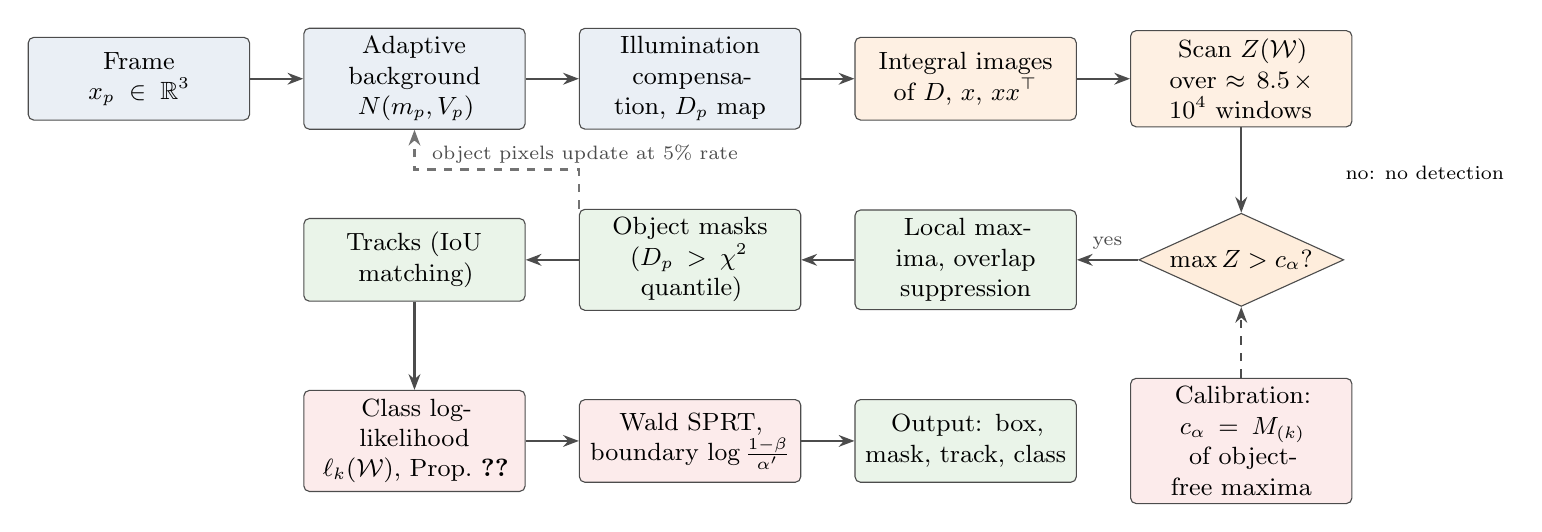
\begin{tikzpicture}[blk/.append style={minimum width=2.7cm,minimum height=1.05cm,text width=2.6cm}]
\node[blk=cA] (frame) at (0,0) {Frame\\$x_p\in\R^3$};
\node[blk=cA] (bg) at (3.5,0) {Adaptive background\\$N(m_p,V_p)$};
\node[blk=cA] (dmap) at (7,0) {Illumination compensation, $D_p$ map};
\node[blk=cB] (ii) at (10.5,0) {Integral images of $D$, $x$, $xx^\top$};
\node[blk=cB] (scan) at (14,0) {Scan $Z(\mathcal W)$ over $\approx8.5\!\times\!10^4$ windows};
\node[dec] (thr) at (14,-2.3) {$\max Z>c_\alpha$?};
\node[blk=cC] (nms) at (10.5,-2.3) {Local maxima, overlap suppression};
\node[blk=cC] (mask) at (7,-2.3) {Object masks ($D_p>\chi^2$ quantile)};
\node[blk=cC] (track) at (3.5,-2.3) {Tracks (IoU matching)};
\node[blk=cR] (cls) at (3.5,-4.6) {Class log-likelihood $\ell_k(\mathcal W)$, Prop.~\ref{prop:window}};
\node[blk=cR] (sprt) at (7,-4.6) {Wald SPRT, boundary $\log\frac{1-\beta}{\alpha'}$};
\node[blk=cC] (out) at (10.5,-4.6) {Output: box, mask, track, class};
\node[blk=cR] (cal) at (14,-4.6) {Calibration: $c_\alpha=M_{(k)}$ of object-free maxima};
\foreach \a/\b in {frame/bg,bg/dmap,dmap/ii,ii/scan,scan/thr,nms/mask,mask/track,track/cls,cls/sprt,sprt/out} \draw[arr] (\a)--(\b);
\draw[arr] (thr)--node[above,font=\scriptsize]{yes}(nms);
\draw[arr,dashed] (cal)--(thr);
\draw[arr,dashed,black!55] (mask.north west) -- ++(0,.5) -| (bg.south);
\node[font=\scriptsize,black!70,anchor=south west] at (3.6,-1.2) {object pixels update at 5\% rate};
\node[font=\scriptsize,anchor=west] at (15.2,-1.2) {no: no detection};
\end{tikzpicture}}
\caption{Pipeline of \swift{}. Blue: per-pixel evidence; orange: scan of all windows, constant time each; green: segmentation and tracking; red: statistical decisions (class evidence and sequential test, and the calibrated threshold). Dashed: the threshold is set from object-free frames; masks feed back to the background update.}
\label{fig:flow}
\end{figure}

\subsection{Constant-time window likelihood}\label{sec:window}
Model the pixels of an object class $k$ as independent $N(\mu_k,\Sigma_k)$.
For a window put $S_1=\sum_{p\in\mathcal W}x_p$ and $S_2=\sum_{p\in\mathcal W}x_px_p^{\top}$.

\begin{proposition}\label{prop:window}
The log-likelihood of the pixels of $\mathcal W$ under class $k$ depends on the data only through $(n,S_1,S_2)$:
\begin{equation}\label{eq:loglik}
\ell_k(\mathcal W)=-\tfrac12\Big[n\big(d\log 2\pi+\log|\Sigma_k|\big)+\tr\!\big(\Sigma_k^{-1}(S_2-S_1\mu_k^{\top}-\mu_kS_1^{\top}+n\mu_k\mu_k^{\top})\big)\Big].
\end{equation}
If the integral images of the $d$ channels $x_i$ and of the $d(d+1)/2$ products $x_ix_j$ are built once per frame, then $(n,S_1,S_2)$ of any window cost four table reads per channel, so $\ell_k(\mathcal W)$ costs $O(d^2)$ operations regardless of $n$.
\end{proposition}
\begin{proof}
Sum the log-density over $\mathcal W$ and expand $(x-\mu)^{\top}\Sigma^{-1}(x-\mu)=x^{\top}\Sigma^{-1}x-2\mu^{\top}\Sigma^{-1}x+\mu^{\top}\Sigma^{-1}\mu$.
The sum of the quadratic form equals $\tr\big(\Sigma^{-1}\sum_p(x_p-\mu)(x_p-\mu)^{\top}\big)$, and $\sum_p(x_p-\mu)(x_p-\mu)^{\top}=S_2-S_1\mu^{\top}-\mu S_1^{\top}+n\mu\mu^{\top}$.
A rectangle sum from an integral image $I$ is $I(y_1,x_1)-I(y_0,x_1)-I(y_1,x_0)+I(y_0,x_0)$.
\end{proof}
\begin{figure}[t]
\centering
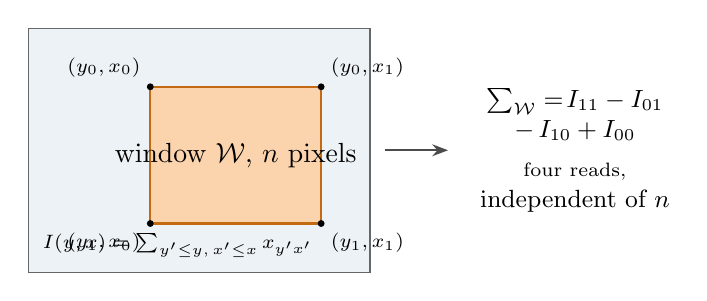
\begin{tikzpicture}[scale=.62]
\fill[cA!10] (0,0) rectangle (7,5); \draw[black!60] (0,0) rectangle (7,5);
\fill[cB!35] (2.5,1) rectangle (6,3.8); \draw[thick,cB!80!black] (2.5,1) rectangle (6,3.8);
\foreach \p in {(2.5,3.8),(6,3.8),(2.5,1),(6,1)} \fill \p circle(2pt);
\node[font=\scriptsize,above left] at (2.5,3.8) {$(y_0,x_0)$}; \node[font=\scriptsize,above right] at (6,3.8) {$(y_0,x_1)$};
\node[font=\scriptsize,below left] at (2.5,1) {$(y_1,x_0)$}; \node[font=\scriptsize,below right] at (6,1) {$(y_1,x_1)$};
\node at (4.25,2.4) {window $\mathcal W$, $n$ pixels};
\node[font=\scriptsize,anchor=south west] at (0.1,0.1) {$I(y,x)=\sum_{y'\le y,\,x'\le x}x_{y'x'}$};
\node[align=center,font=\small] at (11.2,2.5) {$\sum_{\mathcal W}=\!I_{11}-I_{01}$\\$-\,I_{10}+I_{00}$\\[3pt]\scriptsize four reads,\\independent of $n$};
\draw[arr] (7.3,2.5) -- (8.6,2.5);
\end{tikzpicture}
\caption{A rectangle sum from an integral image. The same four reads are used for $\sum x_p$, $\sum x_px_p^\top$ and $\sum D_p$.}
\label{fig:integral}
\end{figure}

\subsection{Motion scan statistic}\label{sec:scan}
Each pixel has an adaptive background $N(m_p,V_p)$ with diagonal $V_p$, updated by exponential forgetting with rate $0.02$; pixels inside detected objects are updated at 5\% of that rate.
A global illumination change must not be mistaken for motion, so the per-channel median of the frame difference is subtracted before scoring and before the variance update.
Let $D_p=(x_p-m_p)^{\top}V_p^{-1}(x_p-m_p)$, capped at a constant to limit the influence of outliers.
On background $D_p$ is approximately $\chi^2_d$, and we define
\begin{equation}\label{eq:Z}
Z(\mathcal W)=\frac{\sum_{p\in\mathcal W}D_p-nd}{\sqrt{2nd}},
\end{equation}
which has mean $0$ and variance $1$ for independent $\chi^2_d$ terms and no cap.
One integral image of $D$ gives $Z(\mathcal W)$ in $O(1)$ for every window.
Windows are taken on a grid of stride $s$, over a geometric set of sizes and three aspect ratios.
For a compact object $Z$ is largest at windows that match it, because added background pixels contribute zero mean and enlarge the denominator.

\subsection{A calibrated threshold over all windows}\label{sec:calibration}
The threshold has to hold for the maximum over the whole window set, not for one window.
Let $M=\max_{\mathcal W}Z(\mathcal W)$ on a frame without moving objects.

\begin{proposition}\label{prop:conformal}
Let $M_1,\dots,M_m$ be the maxima of $m$ object-free frames and $M_{m+1}$ that of a new object-free frame.
If $(M_1,\dots,M_{m+1})$ are exchangeable, and $c$ is the $k$-th smallest of $M_1,\dots,M_m$ with $k=\lceil(m+1)(1-\alpha)\rceil\le m$, then
\begin{equation}
\Pp\big(M_{m+1}>c\big)\le\alpha .
\end{equation}
\end{proposition}
\begin{proof}
By exchangeability, and after breaking ties at random, the rank of $M_{m+1}$ among the $m+1$ values is uniform on $\{1,\dots,m+1\}$.
$M_{m+1}>c$ implies that its rank exceeds $k$, which has probability $(m+1-k)/(m+1)\le\alpha$.
\end{proof}
The bound needs $m\ge\lceil 1/\alpha\rceil-1$ calibration frames and holds whatever the number of windows, their overlap and the distribution of the pixels.
Its assumption is that object-free frames are exchangeable.
With an adaptive background this holds only approximately: the first frames after initialisation are \emph{not} exchangeable with later ones, and the calibration study of Section~\ref{sec:calstudy} shows the consequence, namely a conservative threshold when calibrated early and an anti-conservative one when calibrated after a short burn-in.

\subsection{Segmentation, tracking and sequential classification}\label{sec:track}
All locally maximal windows above the threshold (maximum of $Z$ over a window-sized neighbourhood at each size) are collected.
A greedy suppression keeps the best window and removes every window that overlaps a kept one by at least half of the smaller area, which removes both sub-windows of an object and windows that cover several objects.
Inside a kept window, pixels with $D_p$ above a $\chi^2$ quantile form the object mask.

Detections are matched to existing tracks by intersection over union.
For a track and a frame, the class log-likelihoods of the mask pixels, computed by~\eqref{eq:loglik}, are scaled to $n_{\mathrm{eff}}=20$ effective independent pixels (neighbouring pixels are dependent) and added to the track's accumulated evidence $A(k)$.
With $\lambda(k)=A(k)-\log\sum_{j\ne k}e^{A(j)}$ the log-odds of class $k$ against the rest, class $k$ is declared when $\lambda(k)\ge\log\frac{1-\beta}{\alpha'}$, Wald's upper boundary with error levels $\alpha'=\beta=0.01$.

\subsection{Complexity}\label{sec:complexity}
Per frame the integral images cost $O\big(HW(1+d+d(d+1)/2)\big)$, and each window then costs $O(1)$.
With stride $s$, $S$ sizes and $A$ aspect ratios there are about $(HW/s^2)SA$ windows.
For $320\times240$, $s=4$ and 27 size--shape pairs we score \NwinPerFrame{} windows.
Scanning all windows with $s=1$ and all sizes would need about $(HW)^2/4$ windows, which is not feasible in real time.

\section{Statistical foundations}\label{sec:foundations}
This section fixes the objects of the method as statistical definitions and states what can be proved about them.
Throughout, $\chi^2_\nu$ is the chi-square law with $\nu$ degrees of freedom and $\Pp_0$ the law of an object-free frame.

\begin{definition}[Window family and scan statistic]
Let $\mathcal F$ be a finite set of $N$ windows (rectangles on a stride grid, over a set of sizes and aspect ratios).
For a frame with per-pixel statistics $D_p$ the \emph{scan statistic} is $M=\max_{\mathcal W\in\mathcal F}Z(\mathcal W)$, with $Z$ as in~\eqref{eq:Z}.
\end{definition}

\begin{definition}[Null hypothesis and false-alarm probability]
$H_0$: the frame contains no moving object, and the pixels follow the background, $x_p\sim N(m_p,V_p)$.
For a threshold $c$ the \emph{false-alarm probability per frame} is $\mathrm{FAP}(c)=\Pp_0(M>c)$, the probability that at least one of the $N$ windows exceeds $c$; it is a family-wise error rate over $\mathcal F$.
\end{definition}

\begin{proposition}[Motion statistic as a likelihood-ratio statistic]\label{prop:glr}
Let $V_p$ be known and let the alternative allow every pixel in $\mathcal W$ its own mean. Then the likelihood-ratio statistic of $H_0$ against it is
\[
-2\log\Lambda(\mathcal W)=\sum_{p\in\mathcal W}D_p ,
\]
and under $H_0$ with independent pixels $-2\log\Lambda\sim\chi^2_{nd}$ exactly, so $Z(\mathcal W)$ has mean $0$, variance $1$ and skewness $\sqrt{8/(nd)}$.
\end{proposition}
\begin{proof}
The maximum-likelihood mean of pixel $p$ under the alternative is $x_p$, which makes its log-density $-\tfrac12\log|2\pi V_p|$; under $H_0$ it is lower by $\tfrac12D_p$. Sum over $\mathcal W$. Each $D_p\sim\chi^2_d$ under $H_0$, independent across pixels, so the sum is $\chi^2_{nd}$, with mean $nd$, variance $2nd$ and skewness $\sqrt{8/(nd)}$.
\end{proof}
Thus $\sum D_p$ is not an ad-hoc score: it is the generalised likelihood-ratio statistic, and the standardisation~\eqref{eq:Z} is exact for the moments. The null law of $Z$ is nearly normal only for large $nd$, which is one more reason to calibrate $c$ on the \emph{maximum} instead of using a normal quantile.

\begin{proposition}[Sufficiency]\label{prop:suff}
For independent pixels $N(\mu,\Sigma)$ in a window, $(n,S_1,S_2)$ is a sufficient statistic for $(\mu,\Sigma)$, and minimal sufficient for $n$ fixed.
\end{proposition}
\begin{proof}
By~\eqref{eq:loglik} the joint density factorises as $h(x)\,g_{\mu,\Sigma}(S_1,S_2)$ with $h\equiv(2\pi)^{-nd/2}$; the Fisher--Neyman criterion gives sufficiency. Two samples with the same likelihood ratio for all $(\mu,\Sigma)$ have the same $(S_1,S_2)$ (the exponential family is full rank), which gives minimality.
\end{proof}
This is why the integral images lose no information about the Gaussian window likelihood, for classification as for detection.

\begin{proposition}[Variance under spatial dependence]\label{prop:var}
Let the $D_p$ in $\mathcal W$ have the marginal law $\chi^2_d$ and average pairwise correlation $\bar\rho=\frac{1}{n(n-1)}\sum_{p\ne q}\mathrm{Corr}(D_p,D_q)$. Then
\[
\mathrm{Var}\,Z(\mathcal W)=1+(n-1)\bar\rho,\qquad n_{\mathrm{eff}}=\frac{n}{1+(n-1)\bar\rho}\;\xrightarrow{\,n\to\infty\,}\;\frac1{\bar\rho}.
\]
\end{proposition}
\begin{proof}
$\mathrm{Var}\sum_pD_p=\sum_p\mathrm{Var}\,D_p+\sum_{p\ne q}\mathrm{Cov}(D_p,D_q)=2nd+n(n-1)\bar\rho\,2d$; divide by $2nd$.
\end{proof}
With $\bar\rho>0$, the nominal normal quantiles of $Z$ are too small, and increasingly so for large windows; this is the cause of the failure of the fixed threshold $Z>3$ that we observe, and it is the reason why the effective sample size used in the sequential test is set to $n_{\mathrm{eff}}=20$ instead of the number of mask pixels (an average correlation of about $0.05$ corresponds to $n_{\mathrm{eff}}\to20$).

\begin{proposition}[Localisation]\label{prop:loc}
Suppose an object occupies a set $O$ of $|O|$ pixels on which $\mathrm{E}\,D_p=d+\delta$ with $\delta>0$, and $\mathrm{E}\,D_p=d$ elsewhere. Then for every window, $\mathrm{E}\,Z(\mathcal W)\le\delta\sqrt{|O|/(2d)}$, with equality if and only if $\mathcal W=O$.
\end{proposition}
\begin{proof}
$\mathrm{E}\,Z(\mathcal W)=\delta|\mathcal W\cap O|/\sqrt{2d|\mathcal W|}$. Since $|\mathcal W\cap O|\le\min(|\mathcal W|,|O|)$, we have $|\mathcal W\cap O|/\sqrt{|\mathcal W|}\le\sqrt{|\mathcal W\cap O|}\le\sqrt{|O|}$, and both inequalities are equalities only if $\mathcal W\subseteq O$ and $O\subseteq\mathcal W$.
\end{proof}
Figure~\ref{fig:loc} shows the mean of $Z$ for nested windows around one object: it rises up to the object, then falls as background pixels dilute it. This justifies selecting local maxima of $Z$ across window sizes as object boxes, and shows that the statistic is largest for a window that equals the object, as far as the grid allows.

\begin{figure}[t]
\centering
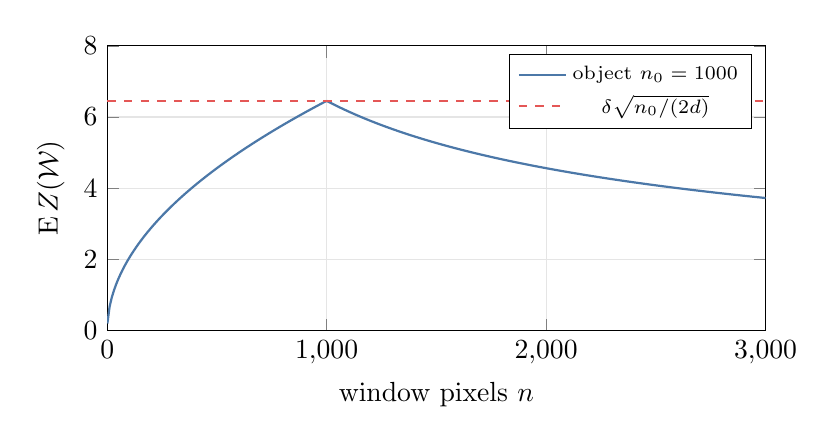
\begin{tikzpicture}
\begin{axis}[width=.82\linewidth,height=5.2cm,xlabel={window pixels $n$},ylabel={$\mathrm{E}\,Z(\mathcal W)$},xmin=0,xmax=3000,ymin=0,ymax=8,xtick={0,1000,2000,3000},
 grid=both,grid style={black!10},legend style={font=\scriptsize,at={(.98,.97)},anchor=north east},every axis plot/.append style={thick}]
\addplot[cA,domain=1:1000,samples=100]{0.5*x/sqrt(6*x)};
\addplot[cA,domain=1000:3000,samples=100,forget plot]{0.5*1000/sqrt(6*x)};
\addplot[cR,dashed,domain=1:3000,samples=2]{0.5*sqrt(1000/6)};
\legend{object $n_0=1000$, $\delta\sqrt{n_0/(2d)}$}
\end{axis}
\end{tikzpicture}
\caption{Proposition~\ref{prop:loc} for $d=3$, an object of $n_0=1000$ pixels and mean excess $\delta=0.5$ of $D_p$ over its null mean. Inside the object $\mathrm{E}\,Z\propto\sqrt n$; once the window is larger than the object, $\mathrm{E}\,Z\propto n^{-1/2}$.}
\label{fig:loc}
\end{figure}

\begin{proposition}[Exact law of the achieved false-alarm probability]\label{prop:beta}
Let $M_1,\dots,M_m$ be i.i.d.\ with continuous distribution function $F$, let $c=M_{(k)}$ be the $k$-th order statistic and $U=1-F(c)$ the false-alarm probability that $c$ actually achieves on a fresh frame. Then $U\sim\mathrm{Beta}(m+1-k,\,k)$, with mean $(m+1-k)/(m+1)\le\alpha$ for $k=\lceil(m+1)(1-\alpha)\rceil$.
\end{proposition}
\begin{proof}
$F(M_{(k)})$ is the $k$-th order statistic of $m$ uniform variables, which has the law $\mathrm{Beta}(k,m+1-k)$; take $1-$ of it.
\end{proof}
Proposition~\ref{prop:conformal} bounds only the \emph{average} of $U$ over calibration samples. A single calibration sample gives a $U$ that varies: for $m=100$ and $\alpha=0.05$ we have $k=96$ and $U\sim\mathrm{Beta}(5,96)$, with mean $0.0495$, standard deviation $0.0215$ and 5\%/95\% quantiles $0.020$/$0.089$. Calibrating on more frames narrows this; the relative standard deviation is about $1/\sqrt{\alpha m}$. Section~\ref{sec:calstudy} compares these values with measurements.

\begin{proposition}[Sequential test: error and delay]\label{prop:wald}
Let the decision rule stop when the log-odds first crosses $A=\log\frac{1-\beta}{\alpha'}$ (declare) or $-B$, $B=\log\frac{1-\alpha'}{\beta}$ (reject). For i.i.d.\ increments Wald's inequalities give actual error levels $\alpha_{\mathrm a}\le\alpha'/(1-\beta)$, $\beta_{\mathrm a}\le\beta/(1-\alpha')$ and $\alpha_{\mathrm a}+\beta_{\mathrm a}\le\alpha'+\beta$, and the expected number of frames under the true class is approximately
\[
\mathrm{E}\,N\approx\frac{A}{n_{\mathrm{eff}}\,\mathrm{KL}},\qquad \mathrm{KL}=\tfrac12(\mu_k-\mu_j)^{\top}\Sigma^{-1}(\mu_k-\mu_j)
\]
per pixel, for Gaussian classes with common covariance (ignoring the overshoot over the boundary).
\end{proposition}
The Kullback--Leibler divergence between $N(\mu_k,\Sigma)$ and $N(\mu_j,\Sigma)$ is half the squared Mahalanobis distance of the means, and the accumulated log-likelihood ratio drifts by $n_{\mathrm{eff}}\mathrm{KL}$ per frame. Table~\ref{tab:asn} compares this approximation with the decision times in Table~\ref{tab:class}. The approximation is in the right range for the two easy separations, where the first frame already crosses the boundary (one frame at least), and gives $2.2$ against $3.9$ at the hardest one; the difference is expected from the overshoot, from the dependence between frames, and from track and mask errors that perturb the increments, none of which the approximation includes. The error levels of the test are not guaranteed here, since the frames of a track are dependent and the scaling $n_{\mathrm{eff}}$ is a device.

\begin{table}[t]
\centering\small
\resizebox{\textwidth}{!}{\begin{tabular}{lccccc}\toprule
Separation & KL (closest pair) & KL (mean pair) & Drift per frame & Predicted $\mathrm{E}[N]$ & Observed \\\midrule
1 & 10.434 & 12.121 & 208.7 & 1.00 & 1.01 \\
0.25 & 0.652 & 0.758 & 13.0 & 1.00 & 1.11 \\
0.1 & 0.104 & 0.121 & 2.1 & 2.20 & 3.91 \\
\bottomrule\end{tabular}
}
\caption{Predicted expected decision time of the sequential test, $\max\{1,A/(n_{\mathrm{eff}}\mathrm{KL})\}$ with the KL of the closest pair of classes, against the observed mean number of frames (Table~\ref{tab:class}). Per-pixel colour sd is $22$, $n_{\mathrm{eff}}=20$, $A=\log 99$.}
\label{tab:asn}
\end{table}

\paragraph{Evaluation measures.}
A detection and a true box match if their intersection over union is at least $0.5$, each true box being used once. With $TP$, $FP$, $FN$ the numbers of matched detections, unmatched detections and unmatched true boxes: precision $=TP/(TP+FP)$, recall $=TP/(TP+FN)$, $F_1=2TP/(2TP+FP+FN)$. The empirical false-alarm rate is the share of object-free frames with at least one detection. Comparisons between methods use the \emph{same} scenes, so we report paired differences with a $t$-interval and the Wilcoxon signed-rank test, which does not assume normal differences; with ten scenes the smallest possible two-sided $p$ is $0.002$. When no false alarm is observed in $n$ trials, the one-sided 95\% Clopper--Pearson upper bound on the probability is $1-0.05^{1/n}\approx3/n$ (the ``rule of three''): for $n=1000$ it is $0.003$, but the frames of one stream are dependent, so it is a bound for the stream, not for independent frames.

\section{Experiments}\label{sec:experiments}
All experiments are on synthetic scenes with exact ground truth.
They check the method against its own assumptions; they are not evidence of performance on real video.

\subsection{Setup}\label{sec:setup}
The simulator renders $320\times240$ colour frames: a smooth random background, additive Gaussian pixel noise (sd 5), a slow sinusoidal illumination drift (amplitude 6 grey levels), and three elliptical objects (28 to 64 pixels across) that bounce at constant speed.
Objects belong to three classes (red, green, yellow) whose pixels are independent Gaussian with overlapping colour distributions (per-channel sd 22).
A parameter, the class separation, pulls the three class means towards their common mean: 1 is the default, $0.25$ and $0.1$ make the classes much harder to tell apart.
Detections match a true box at intersection over union $\ge 0.5$.
Settings were not varied: $\alpha=0.05$, stride $4$, 27 window shapes, $n_{\mathrm{eff}}=20$, Wald levels $0.01$.
Timings are per frame, on two CPU cores of a cloud container, include all stages, and are single-run means over the scene.

\paragraph{Protocol.}
For each scene the threshold is calibrated on 100 object-free frames that follow a 30-frame warm-up; false alarms are counted on the next 100 object-free frames of the same stream; then the 240-frame scene with objects is processed with the same detector.
The results below are on \nSeeds{} scenes (seeds \seedLow--\seedHigh) that were generated after the last change to the algorithm.
The development history, including an earlier run on other scenes that exposed a defect, is in Appendix~\ref{app:history}.

\subsection{Exactness of the window likelihood}\label{sec:exactness}
On random data ($d=3$, window $37\times31$), the log-likelihood from integral images and the direct sum differ by $9\times10^{-13}$ on a value of about $-6156$, which is floating-point precision; this is also an automated test.
Building the nine integral images (three channels, six products) of a $640\times480$ frame takes about 8 ms in our environment.

\subsection{False alarms}\label{sec:false-alarms}
Table~\ref{tab:detection} (column ``False-alarm rate'') gives the share of the 100 object-free test frames that contain at least one detection, averaged over the \nSeeds{} scenes.
With the calibrated threshold no frame raised an alarm in $1000$ frames, against a target of $\alpha=0.05$ (one-sided 95\% upper bound $0.003$ for the stream, Section~\ref{sec:foundations}).
This does \emph{not} show that the bound of Proposition~\ref{prop:conformal} holds: the calibration frames lie early in the stream, when the background has just been initialised from 30 frames, so their maxima are larger than later ones and the threshold is too high. Section~\ref{sec:calstudy} measures this directly and finds an exceedance of $0.000$ in this protocol and of $0.100$ if the threshold is instead calibrated after 100 burn-in frames.
A conventional fixed threshold of $Z>3$ is useless here: it raises an alarm in every frame (rate $1.000$) and its precision falls to $0.06$.
Without the illumination compensation of Section~\ref{sec:scan} the rate is \faNoComp{}: the slow drift of the scene is read as motion by large windows.

\subsection{Detection compared with background subtraction}\label{sec:detection}
\begin{table}[t]
\centering\small
\resizebox{\textwidth}{!}{\begin{tabular}{lccccc}\toprule
Method & Precision & Recall & F$_1$ & False-alarm rate & ms/frame \\\midrule
SWIFT-MO (calibrated) & 0.873$\,\pm\,$0.085 & 0.779$\,\pm\,$0.112 & 0.823$\,\pm\,$0.099 & 0.000 & 5.3$\,\pm\,$0.5 \\
fixed threshold Z>3 & 0.063$\,\pm\,$0.009 & 0.777$\,\pm\,$0.111 & 0.116$\,\pm\,$0.016 & 1.000 & 20.3$\,\pm\,$2.6 \\
no illumination compensation & 0.859$\,\pm\,$0.099 & 0.770$\,\pm\,$0.120 & 0.811$\,\pm\,$0.109 & 0.527 & 4.4$\,\pm\,$0.5 \\
no overlap suppression & 0.026$\,\pm\,$0.007 & 0.974$\,\pm\,$0.017 & 0.050$\,\pm\,$0.013 & 0.000 & 115.4$\,\pm\,$66.5 \\
MOG2 & 0.926$\,\pm\,$0.051 & 0.793$\,\pm\,$0.107 & 0.853$\,\pm\,$0.085 & 0.000 & 1.7$\,\pm\,$0.3 \\
KNN & 0.926$\,\pm\,$0.051 & 0.792$\,\pm\,$0.107 & 0.853$\,\pm\,$0.085 & 0.000 & 2.3$\,\pm\,$0.3 \\
\bottomrule\end{tabular}
}
\caption{Detection on \nSeeds{} held-out synthetic scenes (mean $\pm$ sd over scenes). SWIFT-MO rows are the full method and three ablations; MOG2 and KNN are OpenCV background subtractors followed by a morphological opening and connected components (minimum area 150 pixels). The baselines give no class labels.}
\label{tab:detection}
\end{table}
Table~\ref{tab:detection} compares the methods.
The full method reaches F$_1$ \fSwift{} ($\pm\fSwiftSd$ over scenes); MOG2 and KNN reach \fMog{} and run 2 to 3 times faster (\msKnn{} and \msMog{} ms against \msSwift{} ms per frame).
So on these scenes, for detection alone, the scan statistic is not better than pixel-wise background subtraction and costs more.
Removing overlap suppression is catastrophic (precision $0.03$, about 100 ms per frame), because each object is then reported by dozens of overlapping windows.

Table~\ref{tab:paired} gives the paired differences. Against MOG2, the loss in F$_1$ ($-0.030$) is not significant with ten scenes (95\% interval from $-0.073$ to $+0.012$, Wilcoxon $p=0.19$), so the data are compatible with equal detection quality; the loss in precision ($-0.053$) is significant at the 5\% level (without correction for the four metrics examined), recall does not differ, and the extra time per frame of $3.6$ ms is clearly different from zero. The scenes are synthetic and share one generator, so the intervals describe variation between scenes of this generator only.

\begin{table}[t]
\centering\small
\begin{tabular}{lccc}\toprule
Metric & Mean difference & 95\% $t$-interval & Wilcoxon $p$ \\\midrule
Precision & -0.053 & [-0.098,\,-0.007] & 0.020 \\
Recall & -0.014 & [-0.053,\,0.026] & 0.557 \\
F$_1$ & -0.030 & [-0.073,\,0.012] & 0.193 \\
ms per frame & 3.56 & [3.22,\,3.90] & 0.002 \\
\bottomrule\end{tabular}

\caption{SWIFT-MO (calibrated) minus MOG2, paired over the \nSeeds{} held-out scenes.}
\label{tab:paired}
\end{table}

\begin{figure}[t]
\centering
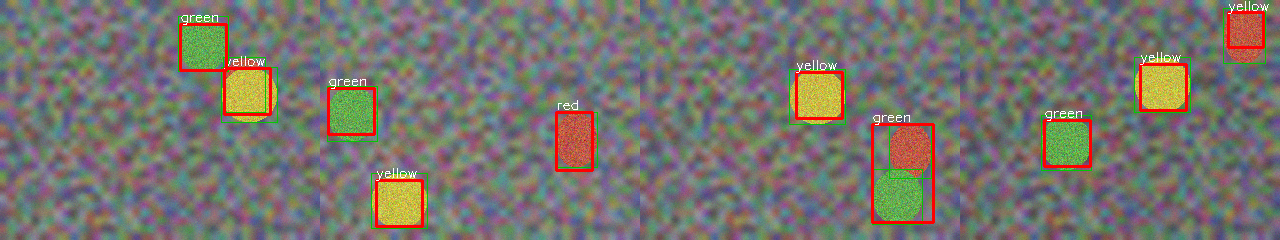
\includegraphics[width=\textwidth]{fig_examples.png}
\caption{Frames 10, 60, 120 and 180 of the development scene. Green: ground truth; red: detections, labelled with the class once the sequential test has decided. Objects appear as textured ellipses because pixels are independent Gaussian.}
\label{fig:examples}
\end{figure}

\subsection{Sequential classification}\label{sec:sprt}
\begin{table}[t]
\centering\small
\resizebox{\textwidth}{!}{\begin{tabular}{rrccccc}\toprule
Class separation & Tracks & Acc.\ after 1 frame & Acc.\ after 5 frames & SPRT decided & SPRT accuracy & SPRT frames \\\midrule
0.1 & 80 & 0.887 & 0.903 & 0.938 & 0.893 & 3.91 \\
0.25 & 85 & 0.847 & 0.895 & 1.000 & 0.835 & 1.11 \\
1 & 77 & 0.870 & 0.870 & 1.000 & 0.818 & 1.01 \\
\bottomrule\end{tabular}
}
\caption{Class decisions per track on the held-out scenes. ``Acc.\ after $n$ frames'' is the accuracy of the class with the largest accumulated log-likelihood after $n$ frames of the track; SPRT is Wald's test with levels $0.01$. Tracks are matched to the true object they overlap most frames.}
\label{tab:class}
\end{table}
Table~\ref{tab:class} compares the sequential test with decisions after a fixed number of frames.
The sequential test is never more accurate than the better of the two fixed rules; at separation $1$ and $0.25$ it decides after about one frame because the evidence accumulated per frame already crosses Wald's boundary, and at separation $0.1$ it needs about four frames to reach an accuracy ($0.89$) close to that of five fixed frames ($0.90$).
Accuracy stays at about $0.82$ to $0.90$ at all separations, including the easiest one, which indicates that most errors come from earlier stages (tracks that merge or swap objects, mask pixels that belong to the background, tracks fragmented across objects) and not from the class models.
We have not isolated these causes, so we claim no benefit of the sequential test here, and its error levels should not be read as guarantees (frames of a track are dependent and the evidence is scaled by $n_{\mathrm{eff}}$).

\subsection{Does the guarantee hold? A calibration study}\label{sec:calstudy}
Proposition~\ref{prop:conformal} requires exchangeable maxima. We test this on 30 further object-free streams (seeds 3000--3029) of $30+B+100+200$ frames: after a 30-frame initialisation, $B$ burn-in frames are discarded, $m=100$ frames calibrate $c$ ($\alpha=0.05$, $k=96$), and 200 later frames measure the achieved exceedance $\widehat U$, the share of their maxima above $c$. We take $B=0$ (the protocol of the benchmark, mode A), $B=100$ (mode B) and $B=300$ (mode C).
Under exchangeability $\widehat U$ has mean $\le0.0495$ and, from Proposition~\ref{prop:beta} and binomial sampling of 200 frames, standard deviation $0.026$.

\begin{table}[t]
\centering\small
\resizebox{\textwidth}{!}{\begin{tabular}{lcccccc}\toprule
Burn-in before calibration & Threshold $c$ & Median $M$ (test) & Max $M$ (test) & Exceedance, mean [95\% CI] & sd & max \\\midrule
A: 0 frames & 14.00 & 5.50 & 7.79 & 0.000 [0.000,\,0.000] & 0.000 & 0.000 \\
B: 100 frames & 6.57 & 5.61 & 7.85 & 0.100 [0.085,\,0.115] & 0.040 & 0.180 \\
C: 300 frames & 6.89 & 5.62 & 7.71 & 0.045 [0.037,\,0.054] & 0.023 & 0.095 \\
Prediction under exchangeability & -- & -- & -- & 0.050 & 0.026 & -- \\
\bottomrule\end{tabular}
}
\caption{Calibration study, 30 streams per row. Threshold and median/maximum of the scan maxima $M$ on the test frames are means over streams; the exceedance is the share of the 200 test maxima above the threshold.}
\label{tab:cal}
\end{table}

\begin{figure}[t]
\centering
\pgfplotsset{calax/.style={width=.355\textwidth,height=4.4cm,xmin=0,xmax=300,ymin=4,ymax=15,xlabel={frame index},tick label style={font=\scriptsize},label style={font=\scriptsize},grid=both,grid style={black!8}}}
\begin{tikzpicture}
\begin{axis}[calax,title={\small A: burn-in 0},ylabel={scan maximum $M$}]
\addplot[only marks,mark=*,mark size=1pt,cA!50] table[x=i,y=m,col sep=space,restrict expr to domain={\thisrow{kind}}{0:0}] {cal_A.dat};
\addplot[only marks,mark=*,mark size=1pt,cA!90!black] table[x=i,y=m,col sep=space,restrict expr to domain={\thisrow{kind}}{1:1}] {cal_A.dat};
\draw[cR,dashed,thick] (axis cs:0,14.27)--(axis cs:300,14.27);
\end{axis}
\end{tikzpicture}\hfill
\begin{tikzpicture}
\begin{axis}[calax,title={\small B: burn-in 100}]
\addplot[only marks,mark=*,mark size=1pt,cB!50] table[x=i,y=m,col sep=space,restrict expr to domain={\thisrow{kind}}{0:0}] {cal_B.dat};
\addplot[only marks,mark=*,mark size=1pt,cB!90!black] table[x=i,y=m,col sep=space,restrict expr to domain={\thisrow{kind}}{1:1}] {cal_B.dat};
\draw[cR,dashed,thick] (axis cs:0,6.42)--(axis cs:300,6.42);
\end{axis}
\end{tikzpicture}\hfill
\begin{tikzpicture}
\begin{axis}[calax,title={\small C: burn-in 300}]
\addplot[only marks,mark=*,mark size=1pt,cC!50] table[x=i,y=m,col sep=space,restrict expr to domain={\thisrow{kind}}{0:0}] {cal_C.dat};
\addplot[only marks,mark=*,mark size=1pt,cC!90!black] table[x=i,y=m,col sep=space,restrict expr to domain={\thisrow{kind}}{1:1}] {cal_C.dat};
\draw[cR,dashed,thick] (axis cs:0,6.81)--(axis cs:300,6.81);
\end{axis}
\end{tikzpicture}
\caption{Scan maxima of stream 3000 under the three calibration modes. Light points: the $m=100$ calibration frames; dark points: the 200 test frames; dashed: the threshold $c$. In mode A the calibration maxima are larger than the test maxima (the background is still settling), so $c$ is far above anything seen later; in mode B the maxima drift upward, so the threshold is too low for the test frames.}
\label{fig:cal}
\end{figure}

The result (Table~\ref{tab:cal}, Figure~\ref{fig:cal}) is in three parts.
(i) Calibrated right after initialisation (A), the threshold is $14.0$ against test maxima of at most $7.8$ on average, and no test frame ever exceeds it: the method is valid but wastes power, since a threshold near $6.9$ would have been enough.
(ii) After 100 burn-in frames (B), the exceedance is $0.100$ (95\% interval $0.085$ to $0.115$), twice the target: the guarantee is \emph{violated}. The cause is visible in Figure~\ref{fig:cal}: the maxima keep rising slowly after the calibration window as the per-pixel variances adapt, which breaks exchangeability in the anti-conservative direction.
(iii) After 300 burn-in frames (C), the exceedance is $0.045$ ($0.037$ to $0.054$) with standard deviation $0.023$, close to the values $0.0495$ and $0.026$ expected from Proposition~\ref{prop:beta} and binomial sampling, so the guarantee holds in practice once the background has settled.
The practical rule is therefore to calibrate only after the background statistics have stabilised, and to monitor the exceedance on later object-free frames.
These are synthetic streams with a stationary drift; real video with slow scene changes can break exchangeability in either direction.

\subsection{A trained detector, for scale only}\label{sec:face}
In an earlier experiment of the same package on a different task (faces in $640\times480$ video), the UltraLight RFB detector took $13.7$ ms per frame and the Haar cascade $100.9$ ms on a Colab CPU.
The tasks, frame sizes, objects and machines differ, so this is not a comparison.
No trained detector has been run on the scenes of this paper.

\section{Discussion}\label{sec:discussion}
\paragraph{What the results support.}
(i) Window likelihoods from integral images are exact and cheap, so a scan over about $8.5\times10^4$ windows fits in a few milliseconds per $320\times240$ frame.
(ii) A threshold taken from the null maxima is necessary: a conventional fixed threshold fails completely on the same data. It keeps false alarms at the target only if the calibration frames are exchangeable with later ones: it did after 300 burn-in frames ($0.045$ against $0.05$), it was twice too permissive after 100 ($0.100$), and it was very conservative when calibrated at once after initialisation ($0.000$).
(iii) Compensation for global illumination matters when the scene drifts.
(iv) Overlap suppression is essential.

\paragraph{What they do not support.}
The method is not more accurate than MOG2/KNN for detection and is slower; the sequential test brought no gain in accuracy; the guarantee was checked only on stationary synthetic streams, and it failed when the calibration window was too early.
The only advantages left are the class labels that the baselines do not provide and the calibrated, interpretable threshold, and the former was shown only on colour-coded synthetic objects.

\paragraph{Assumptions that can fail on real video.}
\begin{itemize}[leftmargin=*,itemsep=2pt]
\item \emph{Pixel model.} Independent Gaussian pixels are wrong for natural images (correlated noise, texture, shadows); then $Z$ is not centred and scaled as in~\eqref{eq:Z}. Proposition~\ref{prop:conformal} does not need the model to be right, which is why the threshold is calibrated, but a wrong model lowers power.
\item \emph{Exchangeability.} Slow drift, camera shake and periodic motion (waves, foliage) violate it, and an adaptive background makes consecutive frames dependent.
\item \emph{Background absorption.} Objects that stop are learned as background; shadows count as motion.
\item \emph{Class models.} Colour alone cannot separate classes of the same colour. Gradients or texture can be added as channels, at the cost of more integral images; not tested.
\item \emph{Tracking.} Overlap-based association fragments tracks; a motion model (Kalman filter) would be a natural improvement.
\item \emph{Window set.} A coarse grid and three aspect ratios limit localisation; very small or elongated objects are missed.
\end{itemize}

\paragraph{Work needed to turn this into a contribution.}
(1) Real video: CDnet~2014 categories, with the object-free segments used to check the false-alarm bound. (2) A trained lightweight detector with a tracker, on the same sequences and one CPU thread. (3) Temporal gating: scan all windows every $m$ frames and only a neighbourhood of predicted boxes otherwise; it is the natural way to gain speed, but it is not implemented, so no gain is claimed. (4) A tracker with a motion model, then re-measurement of the class accuracy to see whether the sequential test helps once upstream errors are removed. (5) Correlated-noise and camera-jitter experiments for the calibration, and an online test of exchangeability (for instance a drift test on the stream of maxima) that decides when calibration may start. (6) A systematic literature search for prior work.

\section{Conclusion}\label{sec:conclusion}
\swift{} scores every sub-window of a frame in constant time from integral images of sufficient statistics, sets its alarm threshold by a finite-sample rank argument that covers all windows at once, and classifies tracked objects sequentially.
On ten held-out synthetic scenes it scans \NwinPerFrame{} windows per $320\times240$ frame in \msSwift{} ms and detects objects with F$_1$ \fSwift{}, slightly below and slower than OpenCV's background subtractors, which give no classes.
A separate calibration study shows that the false-alarm bound holds in practice ($0.045$ against $0.05$) when the threshold is calibrated after the background has settled, fails by a factor two after a short burn-in, and is conservative when calibrated at once. The calibrated threshold and the illumination compensation are shown to be necessary on these data; the sequential classifier is not shown to help.
Whether the properties survive real video, and how the method compares with trained detectors, remains open, and the experiments that would decide it are listed in Section~\ref{sec:discussion}.

\section*{Reproducibility}
The package \texttt{fastfacetrack} (module \texttt{swift}, \texttt{moving}, \texttt{benchmark}) is at \url{https://github.com/yamenetoo/Fast-Face-tracking}.
The tables of this paper are produced by \texttt{paper/make\_tables.py} and \texttt{paper/make\_stats.py} from \texttt{results/benchmark/*.csv} and \texttt{results/calibration/*.csv} (the latter by \texttt{fastfacetrack.benchmark.run\_calibration\_study}, about 40 minutes); the benchmark is \texttt{fastfacetrack.benchmark.run\_benchmark} (about 12 minutes on two CPU cores).

\appendix
\section{Development history and the earlier run}\label{app:history}
The algorithm was developed on one synthetic scene (seed 0) and on scenes with seeds 50--54 used for false-alarm tests.
Three changes were made after looking at results on that scene: (a) local-maximum selection per window size and overlap suppression, after an early version had precision $0.14$ and recall $0.68$; (b) a false-alarm test that calibrates on the same stream, after a first design that calibrated on one scene and tested on others (which Proposition~\ref{prop:conformal} does not cover) gave $0.10$; (c) the illumination compensation.

A first held-out run on ten scenes (seeds 1000--1009) then gave the results of Table~\ref{tab:v1}.
It exposed a defect: the variance update used the uncompensated difference, so a slow global drift inflated the background variance, which lowered both the null maxima and the power.
In that run the fixed threshold $Z>3$ looked as good as the calibrated one (false-alarm rate $0$), which was an artefact of the inflated variance, not a property of the method.
We corrected the update (the variance now uses the compensated difference) and ran a second held-out evaluation on ten new scenes (seeds \seedLow--\seedHigh), which is the one reported in Section~\ref{sec:experiments}.
Both runs are kept in the repository (\texttt{results/benchmark\_v1}, \texttt{results/benchmark}).

\begin{table}[h]
\centering\small
\resizebox{\textwidth}{!}{\begin{tabular}{lccccc}\toprule
Method & Precision & Recall & F$_1$ & False-alarm rate & ms/frame \\\midrule
SWIFT-MO (calibrated) & 0.892$\,\pm\,$0.086 & 0.815$\,\pm\,$0.137 & 0.850$\,\pm\,$0.111 & 0.000 & 4.7$\,\pm\,$0.5 \\
fixed threshold Z>3 & 0.892$\,\pm\,$0.086 & 0.815$\,\pm\,$0.137 & 0.850$\,\pm\,$0.111 & 0.000 & 5.5$\,\pm\,$0.5 \\
no illumination compensation & 0.882$\,\pm\,$0.091 & 0.807$\,\pm\,$0.136 & 0.841$\,\pm\,$0.113 & 0.529 & 4.6$\,\pm\,$0.5 \\
no overlap suppression & 0.026$\,\pm\,$0.005 & 0.963$\,\pm\,$0.037 & 0.050$\,\pm\,$0.009 & 0.000 & 105.1$\,\pm\,$42.2 \\
MOG2 & 0.937$\,\pm\,$0.051 & 0.813$\,\pm\,$0.136 & 0.868$\,\pm\,$0.101 & 0.000 & 1.8$\,\pm\,$0.2 \\
KNN & 0.937$\,\pm\,$0.051 & 0.813$\,\pm\,$0.136 & 0.868$\,\pm\,$0.101 & 0.000 & 2.4$\,\pm\,$0.2 \\
\bottomrule\end{tabular}
}
\caption{First held-out run (seeds 1000--1009) with the variance defect. Compare the fixed-threshold row with Table~\ref{tab:detection}.}
\label{tab:v1}
\end{table}

\begin{thebibliography}{99}\small
\bibitem{crow1984} F.~C. Crow. Summed-area tables for texture mapping. \emph{SIGGRAPH}, 1984.
\bibitem{glaz2001} J.~Glaz, J.~Naus, S.~Wallenstein. \emph{Scan Statistics}. Springer, 2001.
\bibitem{goyette2012} N.~Goyette, P.-M. Jodoin, F.~Porikli, J.~Konrad, P.~Ishwar. changedetection.net: a new change detection benchmark dataset. \emph{CVPR Workshops}, 2012.
\bibitem{kulldorff1997} M.~Kulldorff. A spatial scan statistic. \emph{Communications in Statistics: Theory and Methods}, 26(6), 1997.
\bibitem{lampert2008} C.~H. Lampert, M.~B. Blaschko, T.~Hofmann. Beyond sliding windows: object localization by efficient subwindow search. \emph{CVPR}, 2008.
\bibitem{lei2018} J.~Lei, M.~G'Sell, A.~Rinaldo, R.~J. Tibshirani, L.~Wasserman. Distribution-free predictive inference for regression. \emph{Journal of the American Statistical Association}, 113(523), 2018.
\bibitem{naus1965} J.~I. Naus. The distribution of the size of the maximum cluster of points on a line. \emph{Journal of the American Statistical Association}, 60(310), 1965.
\bibitem{stauffer1999} C.~Stauffer, W.~E.~L. Grimson. Adaptive background mixture models for real-time tracking. \emph{CVPR}, 1999.
\bibitem{viola2004} P.~Viola, M.~J. Jones. Robust real-time face detection. \emph{International Journal of Computer Vision}, 57(2), 2004.
\bibitem{vovk2005} V.~Vovk, A.~Gammerman, G.~Shafer. \emph{Algorithmic Learning in a Random World}. Springer, 2005.
\bibitem{wald1945} A.~Wald. Sequential tests of statistical hypotheses. \emph{Annals of Mathematical Statistics}, 16(2), 1945.
\end{thebibliography}
\noindent\textit{The reference list was written from memory and has not been checked against the sources; verify authors, years, titles and venues before submission.}

\end{document}
